\documentclass[]{spie}
\usepackage[]{graphicx}
\usepackage{url}
\usepackage[]{amsmath}
% \usepackage{subcaption}
% \usepackage[font=small,labelfont=bf]{caption}

\newcommand{\Lcube}{\boldsymbol L^3}
\newcommand{\XI}{\mathrm{XI}}
\newcommand{\SI}{\mathrm{SI}}
\newcommand{\XIT}{\mathrm{XI_{Tun}}}
\newcommand{\XIF}{\mathrm{XI_{Flu}}}
\newcommand{\SIT}{\mathrm{SI_{Tun}}}
\newcommand{\SIF}{\mathrm{SI_{Flu}}}
\newcommand{\SID}{\mathrm{SI_{D65}}}
\newcommand{\SIE}{\mathrm{SI_{Ens}}}
\newcommand{\SIGT}{\mathrm{SI-T}}
\newcommand{\SITT}{\mathrm{SI_{Tun}-T}}
\newcommand{\SIFT}{\mathrm{SI_{Flu}-T}}
\newcommand{\SIDT}{\mathrm{SI_{D65}-T}}
\newcommand{\SIET}{\mathrm{SI_{Ens}-T}}
\newcommand{\TT}{\mathrm{T}}


\title{Efficient illuminant correction in the Local, Linear, Learned ({\LARGE$\boldsymbol L^3$}) method}

\author{Francois G. Germain\supit{a}, Iretiayo A. Akinola\supit{b}, Qiyuan Tian\supit{b}, Steven Lansel\supit{c}, and Brian A. Wandell\supit{b,d}
\skiplinehalf
\supit{a}Center for Computer Research in Music and Acoustics,\\ Stanford University, Stanford, CA-94305, USA;\\
\supit{b}Electrical Engineering Department, Stanford University, Stanford, CA-94305, USA;\\
\supit{c}Olympus Corporation of the Americas, Sunnyvale, CA-94085, USA;\\
\supit{d}Psychology Department, Stanford University, Stanford, CA-94305, USA.
}

\authorinfo{Send correspondence to Francois G. Germain. E-mail: FG (fgermain@stanford.edu), IA (iakinola@stanford.edu), QT (qytian@stanford.edu), SL (steven.lansel@olympus.com), BW (wandell@stanford.edu)}

\begin{document}
\maketitle

\begin{abstract}

To speed the development of novel camera architectures we proposed a method, $\Lcube$ (Local, Linear and Learned), that uses camera simulation to create an optimized image processing pipeline. The $\Lcube$ method assigns each pixel into one of about 400 classes and uses camera simulation and machine learning to derive a linear transform for the data in each class. Each linear transform maps the sensor data from a pixel and its neighbors into the target output (e.g., image XYZ rendered under a D65 illuminant). The 400 transforms are stored in a table and used for image rendering. The sensor and rendering illuminant can be equal (same-illuminant table) or different (cross-illuminant table). In the original implementation, we derived many cross-illuminant tables, and the collection of tables can be relatively large. We find, however, that a single same-illuminant table (D65) effectively converts sensor data for many different same-illuminant conditions. Hence, we propose to render the data by applying the same-illuminant D65 table to the sensor data, followed by a color correction transform. The mean color reproduction error using the same-illuminant table is on the order of 4$\Delta E$ units, which is only slightly larger than the cross-illuminant table errors. This approach reduces table storage requirements significantly without substantially degrading color reproduction accuracy.

\end{abstract}

\keywords{Local Linear Learned ($\Lcube$), image processing pipeline, illuminant correction }

\section{INTRODUCTION}

The $\Lcube$ algorithm automatically generates a standard image processing pipeline (sensor correction, demosaicking, illuminant correction, noise reduction) for novel camera architectures \cite{Tian2014,Lansel2011a,Lansel2011,Lansel2012}. The $\Lcube$ image processing pipeline comprises two parts \cite{Tian2014}. First, the pipeline classifies each pixel (based on a statistical analysis of the responses at the pixel and its neighborhood) into one of many possible classes. Second, the processing pipeline linearly transforms the data of the pixel and its neighbors to the target output space.

The $\Lcube$ training builds a table of linear transforms from a camera model that is implemented using the Image Systems Engineering Toolbox (ISET) \cite{Farrell2003,Farrell2012}. The simulation converts many samples of natural scenes to sensor data. The desired rendering, i.e. CIE XYZ values for consumer photography, are computed from the known natural scene radiance. Through multiple simulations, the $\Lcube$ algorithm learns a table of linear transforms that convert sensor data to the target CIE XYZ values. 

\section{MOTIVATION: ILLUMINANT CORRECTION}

\begin{figure}
\begin{center}
 \includegraphics[width=\textwidth]{Fig1/illuminant_processing}
\end{center}
\caption{ \textbf{Illuminant correction with $\Lcube$ image processing pipelines.} (a) Cross-illuminant ($\XI$) illuminant-dependent $\Lcube$ processing. (b) Same-illuminant ($\SI$) illuminant-independent $\Lcube$ processing followed by a linear color correction transform ($\TT$).}
\label{fig:sensordisplay}
\end{figure}

Illuminant correction is an essential part of the image processing pipeline that is necessary to account for the perceptual phenomenon of \textit{color constancy} \cite{Wandell1995}. The visual system adapts to changes in the ambient light level and color, and this adaptation has the general effect of preserving the color appearance of an object (e.g. a white shirt) across conditions (daylight to tungsten light). Because the human visual system adapts to the illuminant, to preserve color appearance the linear transforms in the $\Lcube$ method used for rendering must adapt, too.

In the original algorithm, we anticipated learning a table of linear transforms for each illumination condition (cross-illuminant, Figure~\ref{fig:sensordisplay}(a)). These cross-illuminant tables would be stored and applied for rendering. This approach pays a significant cost in computation and storage. Here, we explore an approach that separates illuminant correction from the rest of the pipeline. We learn a same-illuminant table, that renders data acquired under one illuminant into XYZ values under the same illuminant. This accomplishes demosaicking, denoising and sensor correction, but it does not perform illuminant correction (Figure~\ref{fig:sensordisplay}(b)). We then apply an illuminant correction transform to obtain the final rendering. This architecture requires training and storing only one table of $\Lcube$ transforms to be used for all illuminants and one illuminant correction matrix for each illuminant of interest. 

\section{METHOD}

\begin{figure}[t]
 \begin{center}
\begin{minipage}{0.45\textwidth}
\begin{flushright}
 \begin{scriptsize}
\begin{tabular}{|l|c|}
\hline 
\multicolumn{2}{|c|}{\textbf{Optics(diffraction-limited)}} \\\hline 
Focal length(mm) & 3 \\ 
F-number & 4 \\ 
Aperture diameter (mm) & 0.75 \\ \hline 
\multicolumn{2}{|c|}{\textbf{Sensor}} \\ \hline 
Rows/Columns & 204 $\times$ 240 \\ 
Size (mm) & 0.4488 $\times$ 0.528 \\ 
Dark noise nonuniformity (mV) & 1.41 \\ 
Photoreceptor nonuniformity (\% ) & $2.218 \times 10 ^{-3}$ \\ 
Analog gain & 1 \\ 
Analog offset (V) & 0 \\\hline 
\multicolumn{2}{|c|}{\textbf{Sensor pixel }} \\ \hline 
Width/height ($\mu$m) & 2.2 $\times$ 2.2\\ 
Fill factor & 0.45 \\
Dark voltage (V/sec) & $1 \times 10^{-5}$ \\ 
Read noise (mV) & 1.34 \\ 
Conversion gain $(\mu V/e)$ & 200 \\ 
Voltage swing (V) & 1.8 \\ 
Well capacity (electrons) & 9000 \\ \hline 
\end{tabular} 
\end{scriptsize}
\end{flushright}
\end{minipage}\hfill
\begin{minipage}{0.45\textwidth}
\begin{flushleft}
 
\includegraphics[height=5.5cm]{Fig2/chart}
\end{flushleft}
\end{minipage}
\end{center}
\caption{\textbf{Sensor parameter values (left) and Natural-100 color test chart (right)}}
\label{fig:natureBasedChart}
\end{figure}

\subsection{General simulation conditions}

We used ISET \cite{Farrell2003,Farrell2012} to simulate digital camera processing. The ISET camera model includes the simulation of scene radiance, optics, sensor electronics and image processing pipeline (here the $\Lcube$ pipeline). We model the camera as an f/4 lens with diffraction limited optics and focal length of 3mm. The sensor uses a RGB/W color filter array (CFA) layout described in \cite{Tian2014}, with parameter values as in Figure~\ref{fig:natureBasedChart}. 

The $\Lcube$ algorithm uses simulated training data to learn a table of linear transforms \cite{Tian2014}. Each pixel in the simulated sensor data is assigned to a distinct class based on (a) its color type (R, G, B, W), (b) the response voltage level (low, middle, high), and (c) the neighborhood spatial pattern (uniform or textured). The transform for a given class is derived by optimizing a Wiener filter between the data in the pixel neighborhood in the sensor, and the corresponding ideal value in the target color space (XYZ). 

The rendering process identifies the class membership for each pixel in the sensor data and then applies the appropriate stored linear transform. The image processing pipeline, which performs demosaicking, denoising, sensor conversion comprises the application of these precomputed local, linear transforms.

\subsection{Learning the $\Lcube$ tables}

\paragraph{Learning the cross-illuminant tables} Cross-illuminant ($\XI$) tables of $\Lcube$ transforms are learned by simulating the sensor data under tungsten ($\XIT$) and fluorescent ($\XIF$) illumination and rendering to a target representation (XYZ) under a D65 illuminant.

\paragraph{Learning the same-illuminant table} Same-illuminant ($\SI$) tables of $\Lcube$ transforms are learned by simulating sensor data and the target display XYZ values using the same illuminant. We learned same-illuminant tables for D65 ($\SID$), tungsten ($\SIT$) and fluorescent ($\SIF$). To complete the rendering, we apply an illuminant correction transform from the acquisition illuminant to the final D65 rendering. The matrix $\TT$ is derived by a linear regression between the XYZ values in the acquired and target (D65) representations. $\TT$ is derived from first principles and is not dependent on the camera structure or $\Lcube$. 

In principle, any of the SI tables can be used. In fact, it is possible to learn a same-illuminant table using sensor data from an ensemble of illuminants. (e.g., a mixture of D65 and tungsten scenes). The linear transforms reflect the properties of the multiple illuminants used in the ensemble, rather than the requirements of a specific illuminant. For example, the response level of a blue pixel under tungsten illuminant is typically quite low as reflected in the images obtained from tungsten-based table. The $\Lcube$ compensates by using linear transforms with more blurring on those pixels compared to the D65 same-illuminant transforms. We learned tables for an ensemble comprising data from a mixture of D65 and Tungsten illuminants ($\SIE$) which results in a more robust table for both illuminants.

\subsection{Color evaluation} 

To compare the $\XI$ and $\SI$ methods, we used data from hyperspectral scenes and simulated test charts.

\paragraph{Multispectral scenes} We used a small set of multispectral scenes including the Macbeth (Gretag) color chart, fruits, and people \cite{iset}. These images compare the algorithms visually.

\paragraph{Natural-100 reflectance chart} To generate a systematic and quantitative assessment of the color reproduction error, we created a Natural-100 test chart (Figure~\ref{fig:natureBasedChart}). The chart includes 100 samples with natural object reflectances from five categories \cite{Vrhel1994}, and a 10-sample gray color strip. The reflectances are grouped by category (20 food, 20 clothes, 20 nature, 5 hair, 15 skin and 20 paint color samples). To select the category samples we calculated 7 principal components for the entire set of natural reflectances, represented each sample by its component weights, and then formed clusters of the samples. If N samples are needed from a category, we formed N clusters for that category and chose one sample from each cluster. By selecting one sample per cluster per category we ensure that the final chart has a variety of reflectances that span the sample pool.

We quantified color reproduction error using CIE2000 $\Delta E$ units \cite{Sharma2005}. The error was the difference between the chart XYZ under a D65 illuminant and the data rendered using either the $\SI$ or $\XI$ method.

\section{EXPERIMENTAL RESULTS}

\begin{figure}[t]
\begin{center}
\begin{minipage}[b]{0.245\textwidth}
 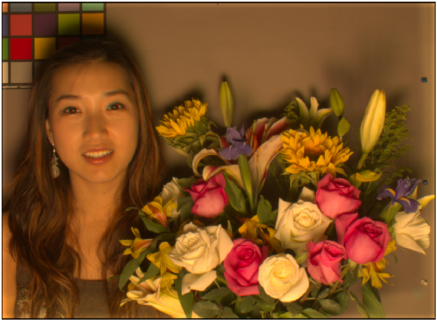
\includegraphics[width=\textwidth]{Fig3/srgbI_AsianFemaleWithFlowers_RGBW1_Tungsten1_opt2}
 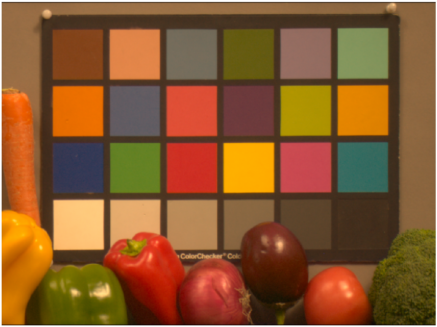
\includegraphics[width=\textwidth]{Fig3/srgbI_Vegetables_RGBW1_Tungsten1_opt2}
 \centering\small\text{(a) Ideal tungsten}
\end{minipage}
\begin{minipage}[b]{0.245\textwidth}
 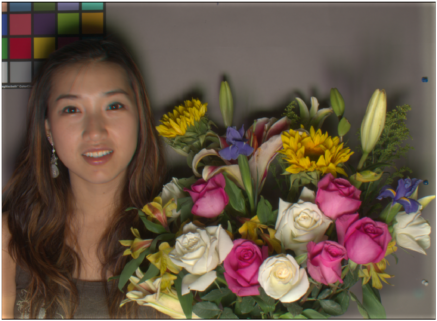
\includegraphics[width=\textwidth]{Fig3/srgbI_AsianFemaleWithFlowers_RGBW1_Tungsten1_opt1}
 
\includegraphics[width=\textwidth]{Fig3/srgbI_Vegetables_RGBW1_Tungsten1_opt1}
 \centering\small\text{(b) Ideal D65}
\end{minipage}
\begin{minipage}[b]{0.245\textwidth}
 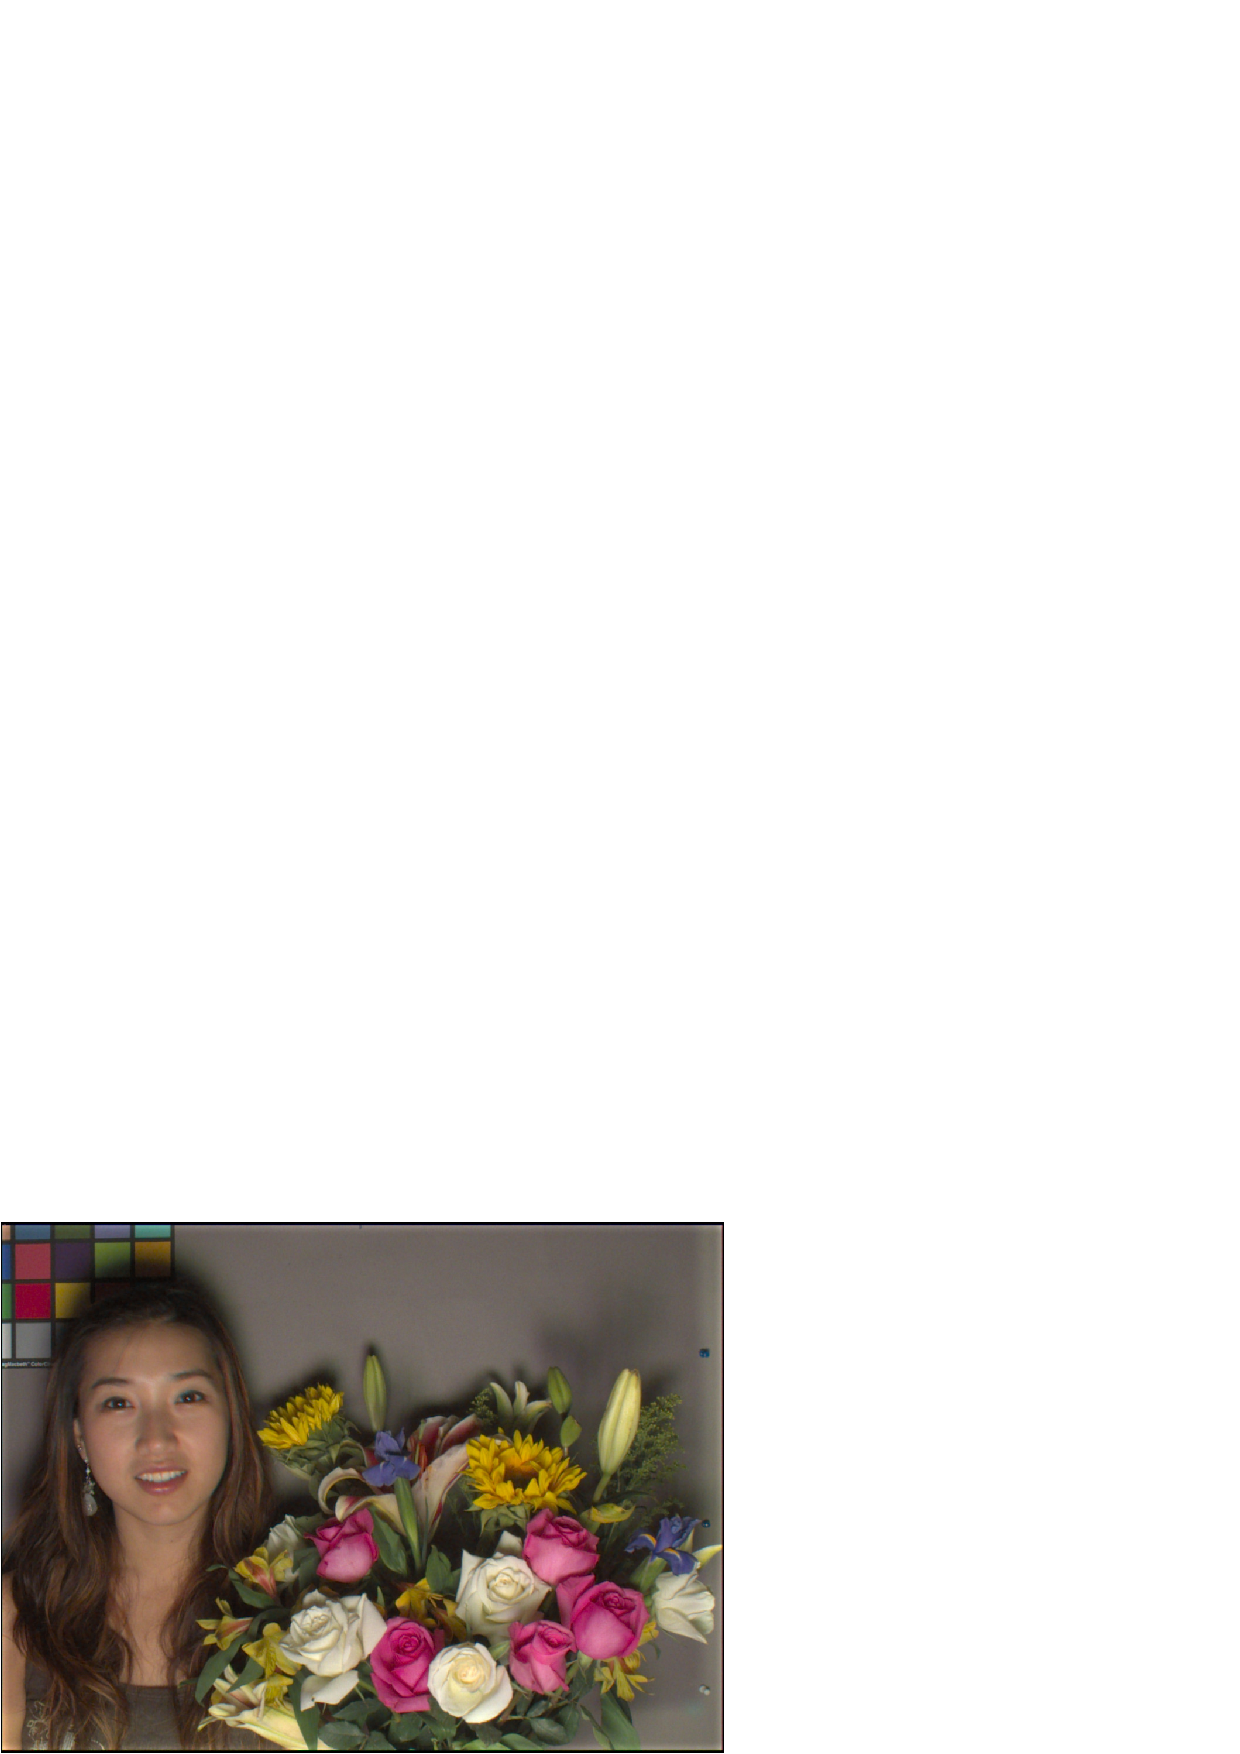
\includegraphics[width=\textwidth]{Fig3/srgbR_AsianFemaleWithFlowers_RGBW1_Tungsten1_opt2}
 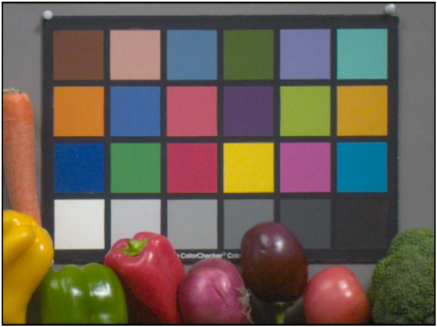
\includegraphics[width=\textwidth]{Fig3/srgbR_Vegetables_RGBW1_Tungsten1_opt2}
 \centering\small\text{(c) $\XIT$}
\end{minipage}
\begin{minipage}[b]{0.245\textwidth}
 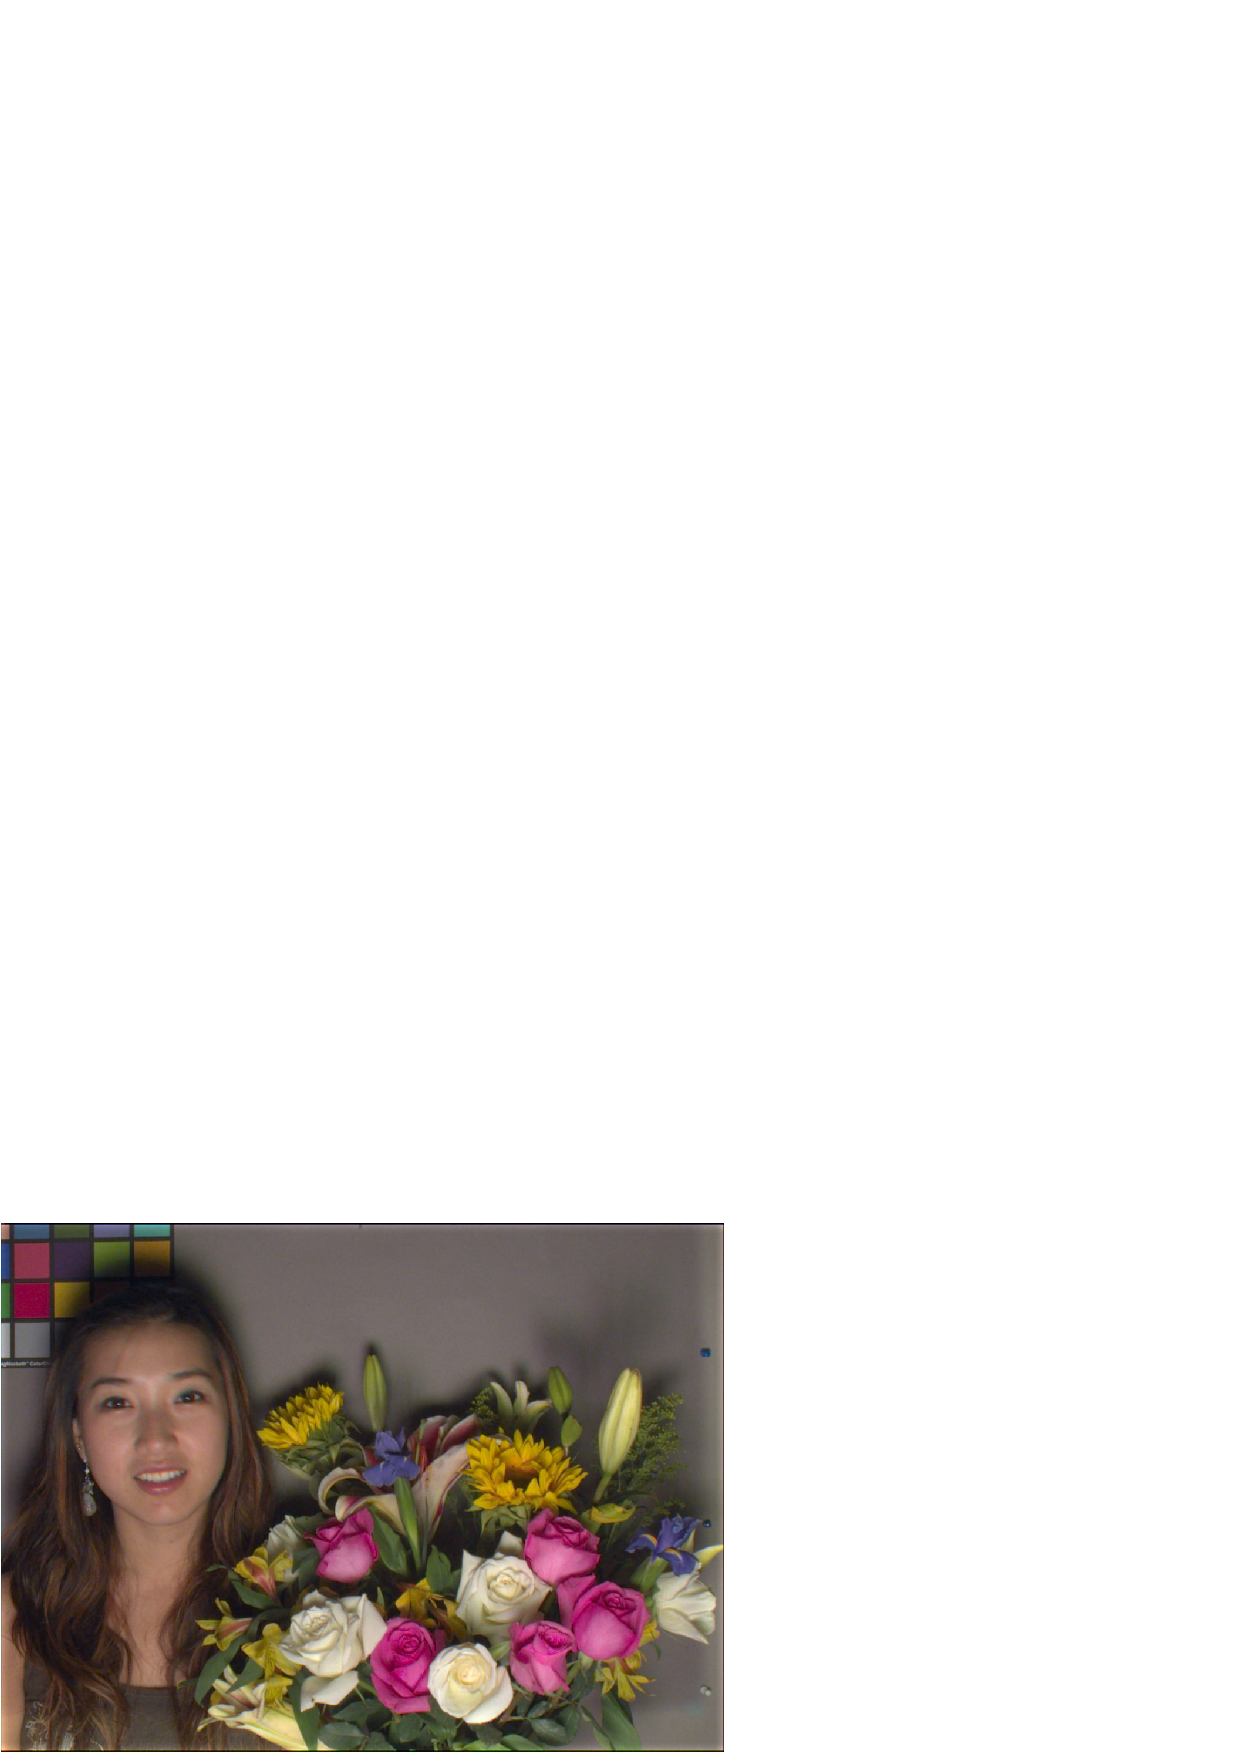
\includegraphics[width=\textwidth]{Fig3/srgbR_AsianFemaleWithFlowers_RGBW1_Tungsten1_opt3}
 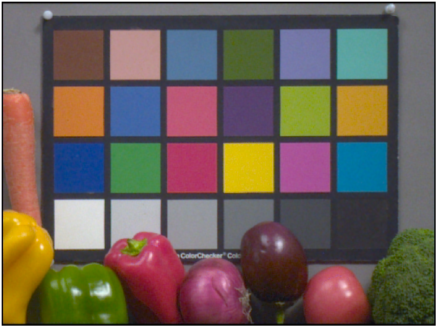
\includegraphics[width=\textwidth]{Fig3/srgbR_Vegetables_RGBW1_Tungsten1_opt3}
 \centering\small\text{(d) $\SIDT$}
\end{minipage}
\end{center}
\caption{\textbf{Cross-illuminant and same-illuminant algorithms perform equally well in color rendering for a tungsten illuminant.} (a) The sensor image under tungsten, uncorrected. (b) The ideal image under a D65 illumination. (c) A cross-illuminant analysis for the same image but acquired under a tungsten light. The $\Lcube$ table was built from the tungsten-acquisition data and XYZ target values for a D65-rendered image. (d) A same-illuminant rendering. In this case the L3 table was built using the same-illuminant D65 table, and the final rendering combined this table with an illuminant correction matrix $\TT$. The cross-illuminant and same-illuminant architectures produce similar images.}
\label{fig:examplestungsten}
\end{figure}

\begin{figure}[t]
\begin{center}
\begin{minipage}[b]{0.245\textwidth}
 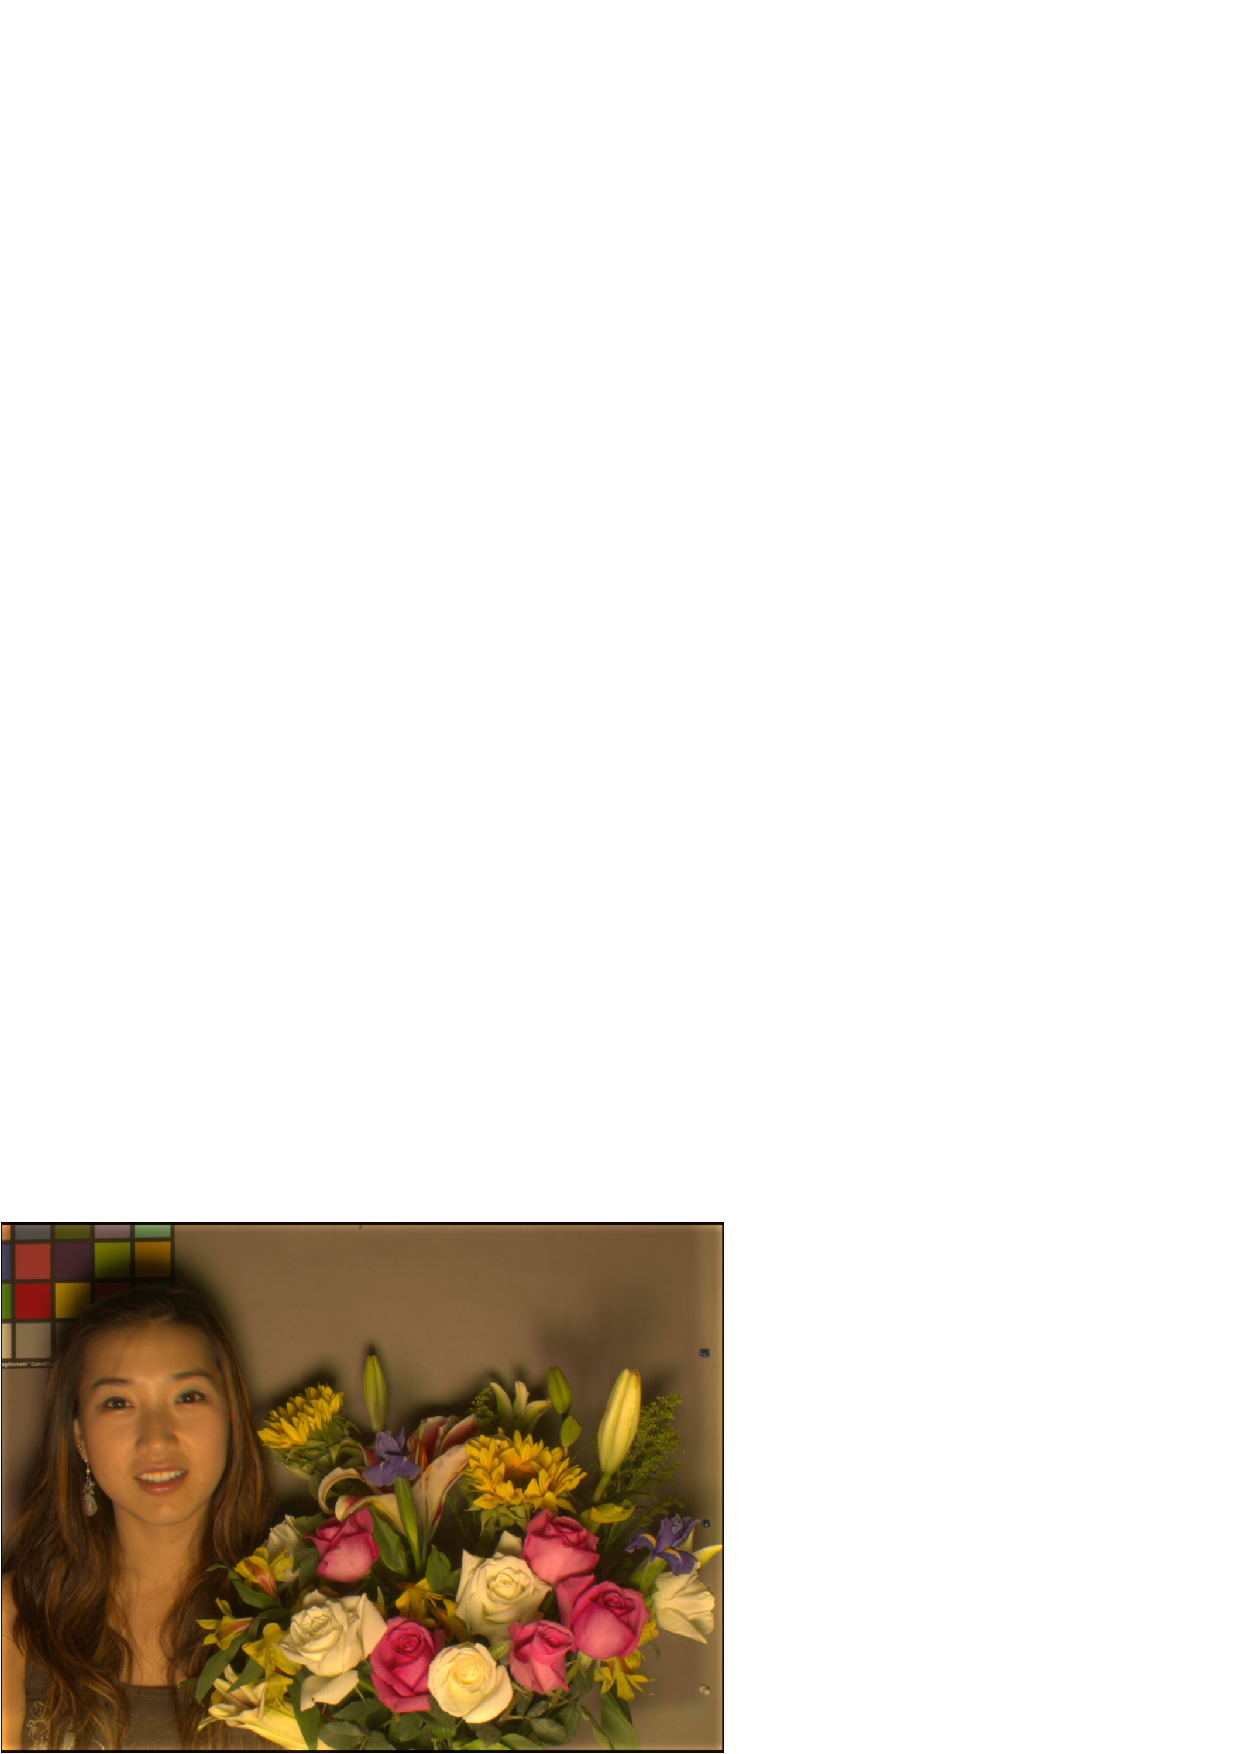
\includegraphics[width=\textwidth]{Fig4/srgbI_AsianFemaleWithFlowers_RGBW1_Fluorescent1_opt2}
 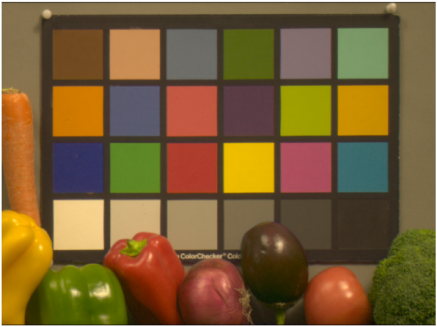
\includegraphics[width=\textwidth]{Fig4/srgbI_Vegetables_RGBW1_Fluorescent1_opt2}
 \centering\small\text{(a) Ideal fluorescent}
\end{minipage}
\begin{minipage}[b]{0.245\textwidth}
 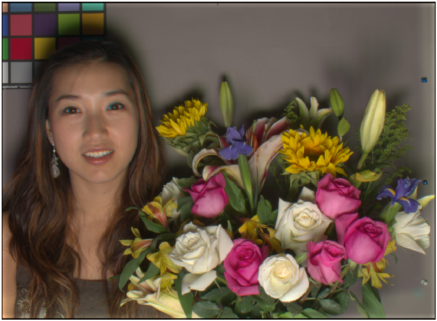
\includegraphics[width=\textwidth]{Fig4/srgbI_AsianFemaleWithFlowers_RGBW1_Fluorescent1_opt1}
 
\includegraphics[width=\textwidth]{Fig4/srgbI_Vegetables_RGBW1_Fluorescent1_opt1}
 \centering\small\text{(b) Ideal D65}
\end{minipage}
\begin{minipage}[b]{0.245\textwidth}
 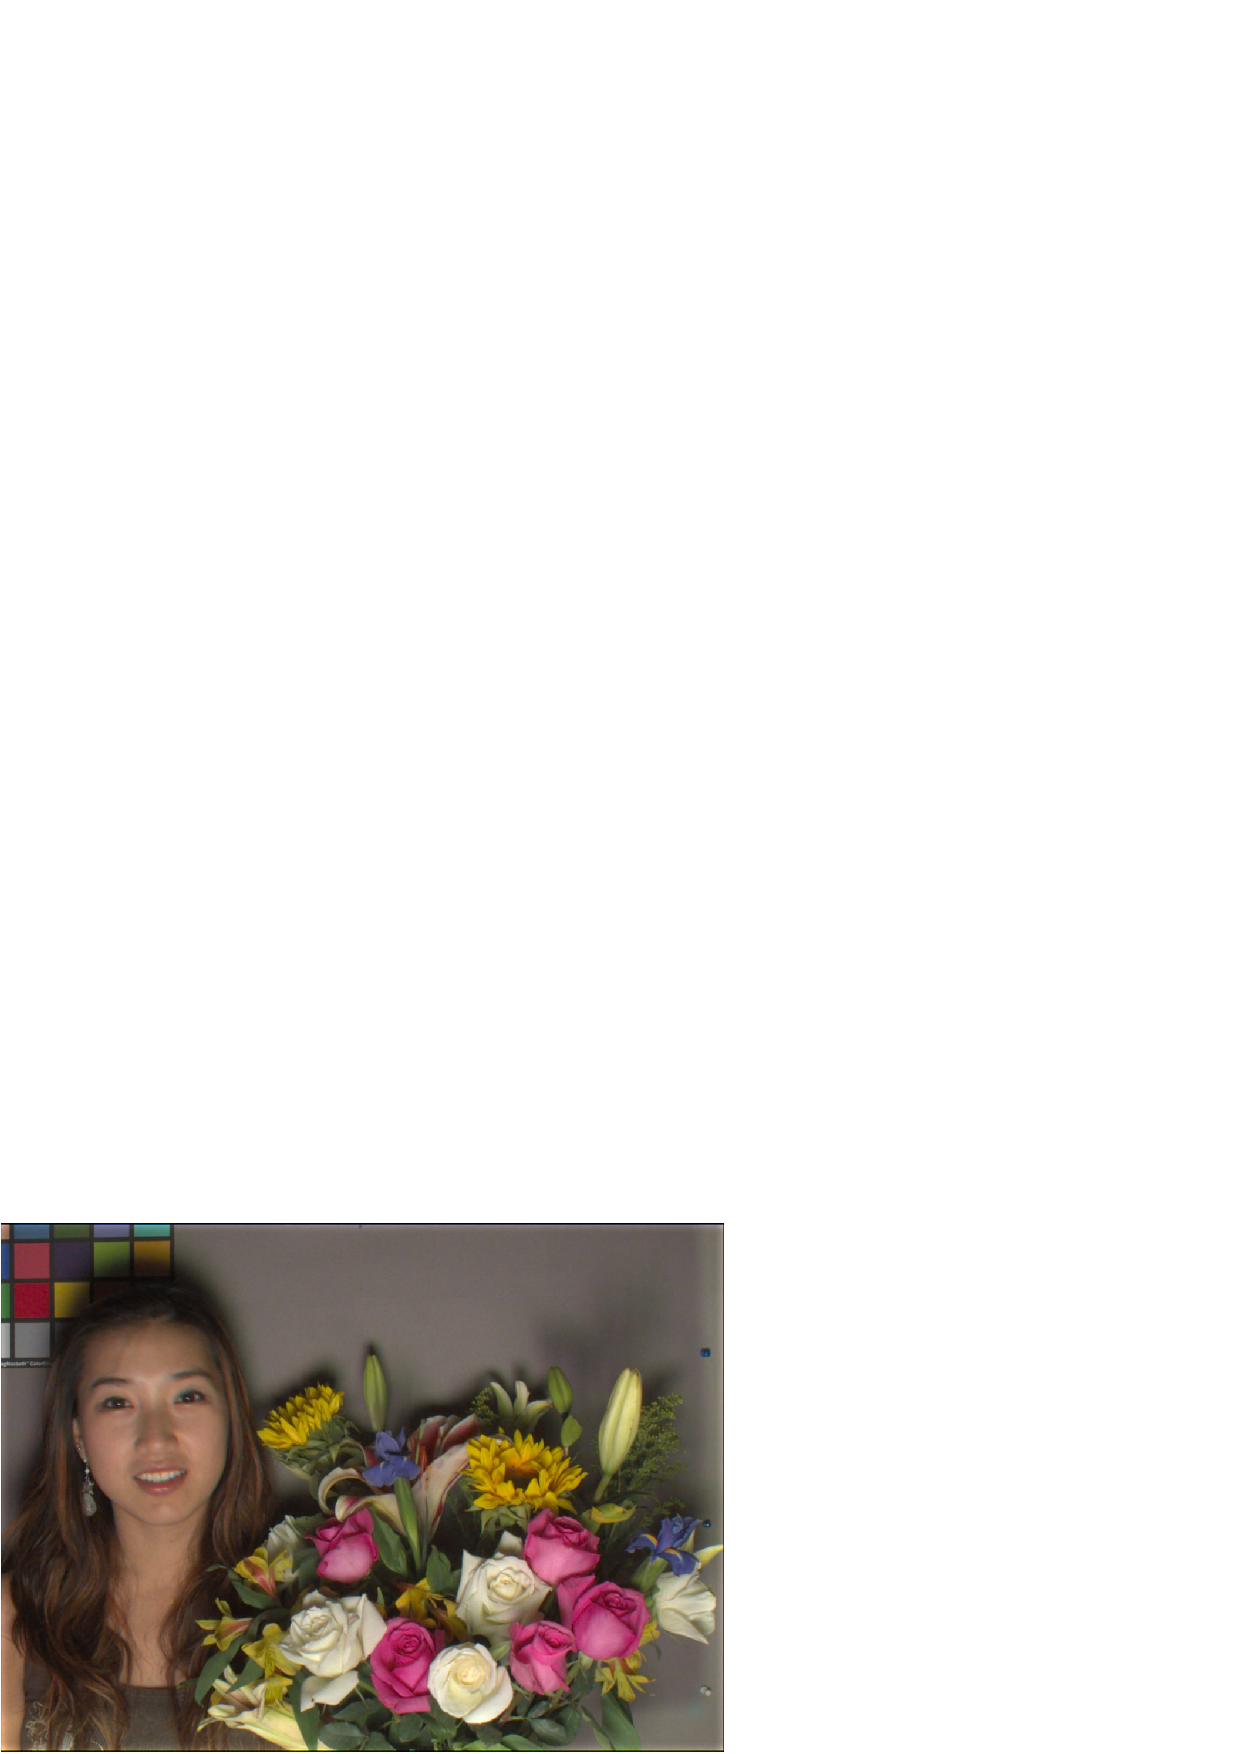
\includegraphics[width=\textwidth]{Fig4/srgbR_AsianFemaleWithFlowers_RGBW1_Fluorescent1_opt2}
 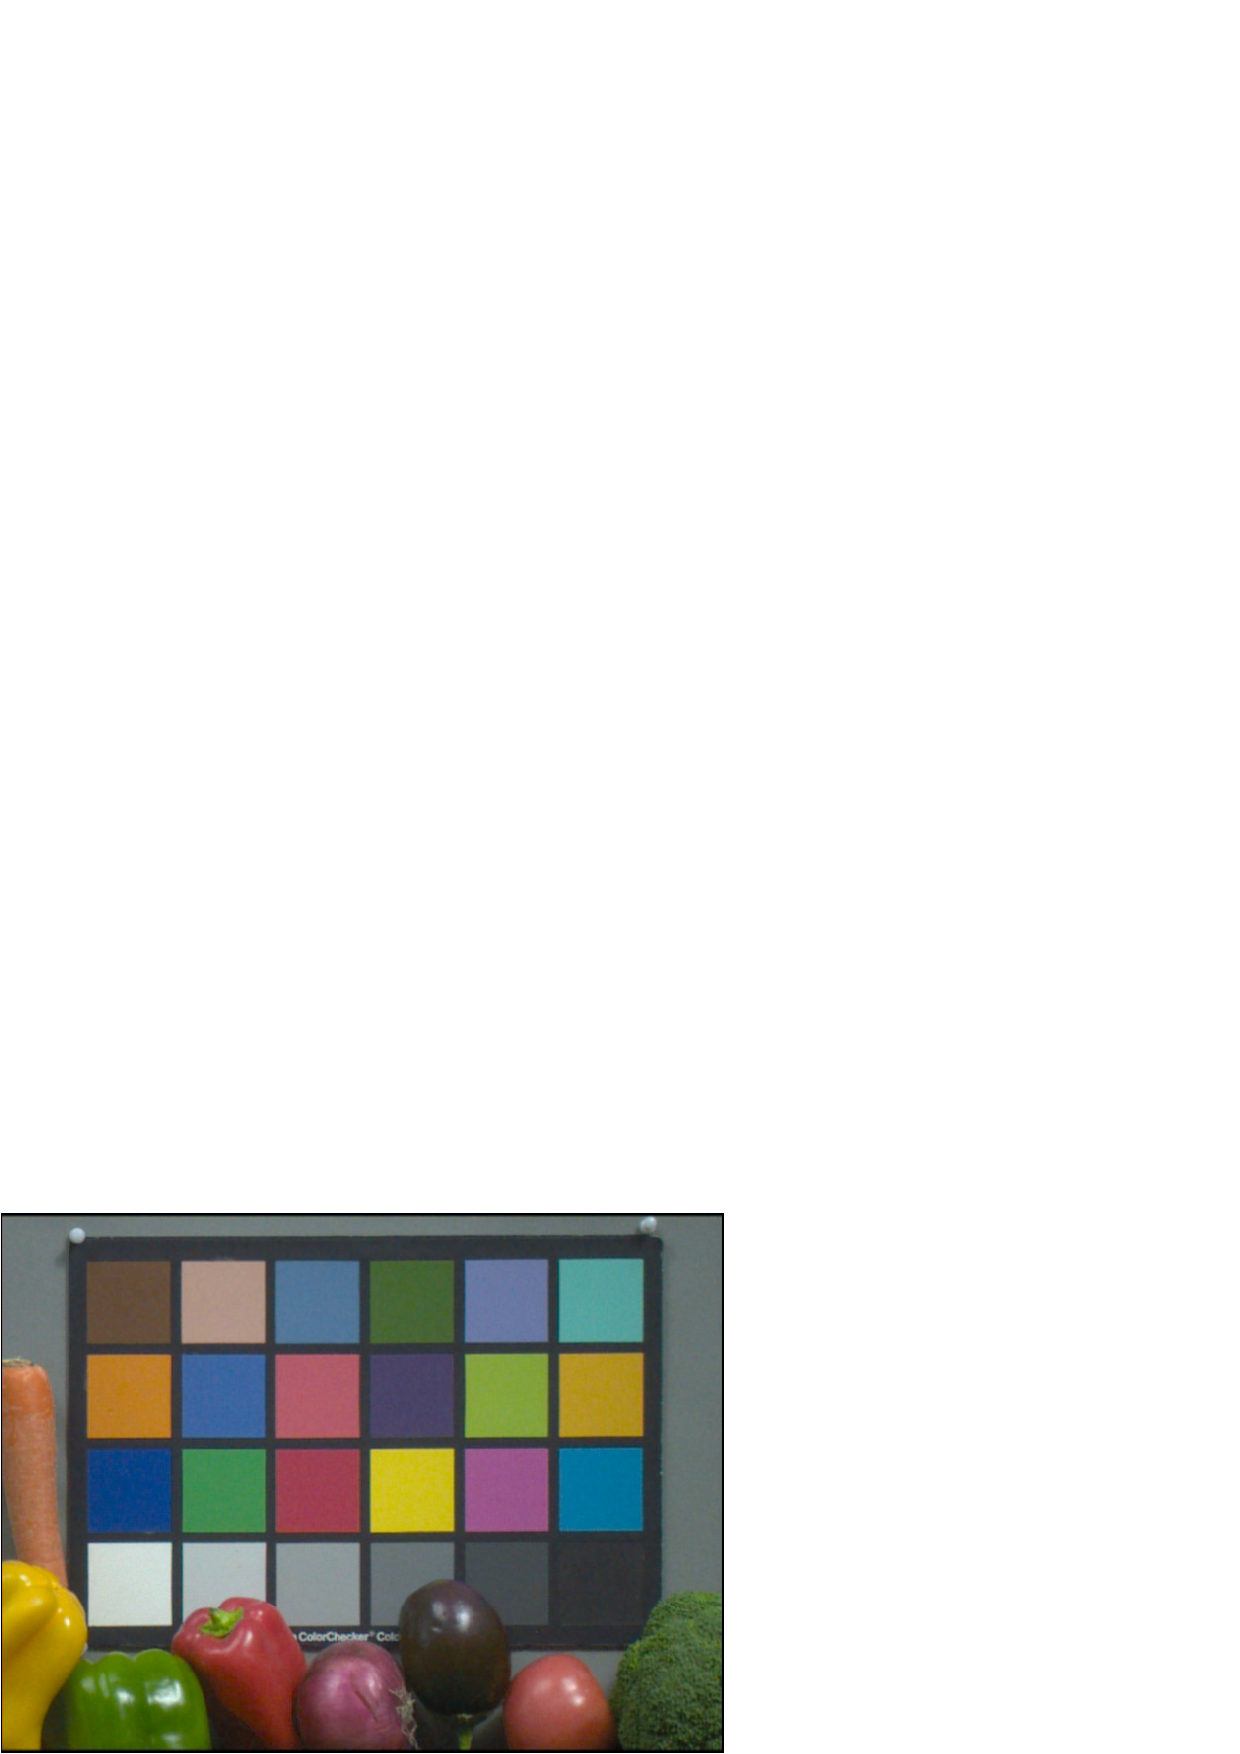
\includegraphics[width=\textwidth]{Fig4/srgbR_Vegetables_RGBW1_Fluorescent1_opt2}
 \centering\small\text{(c) $\XIF$}
\end{minipage}
\begin{minipage}[b]{0.245\textwidth}
 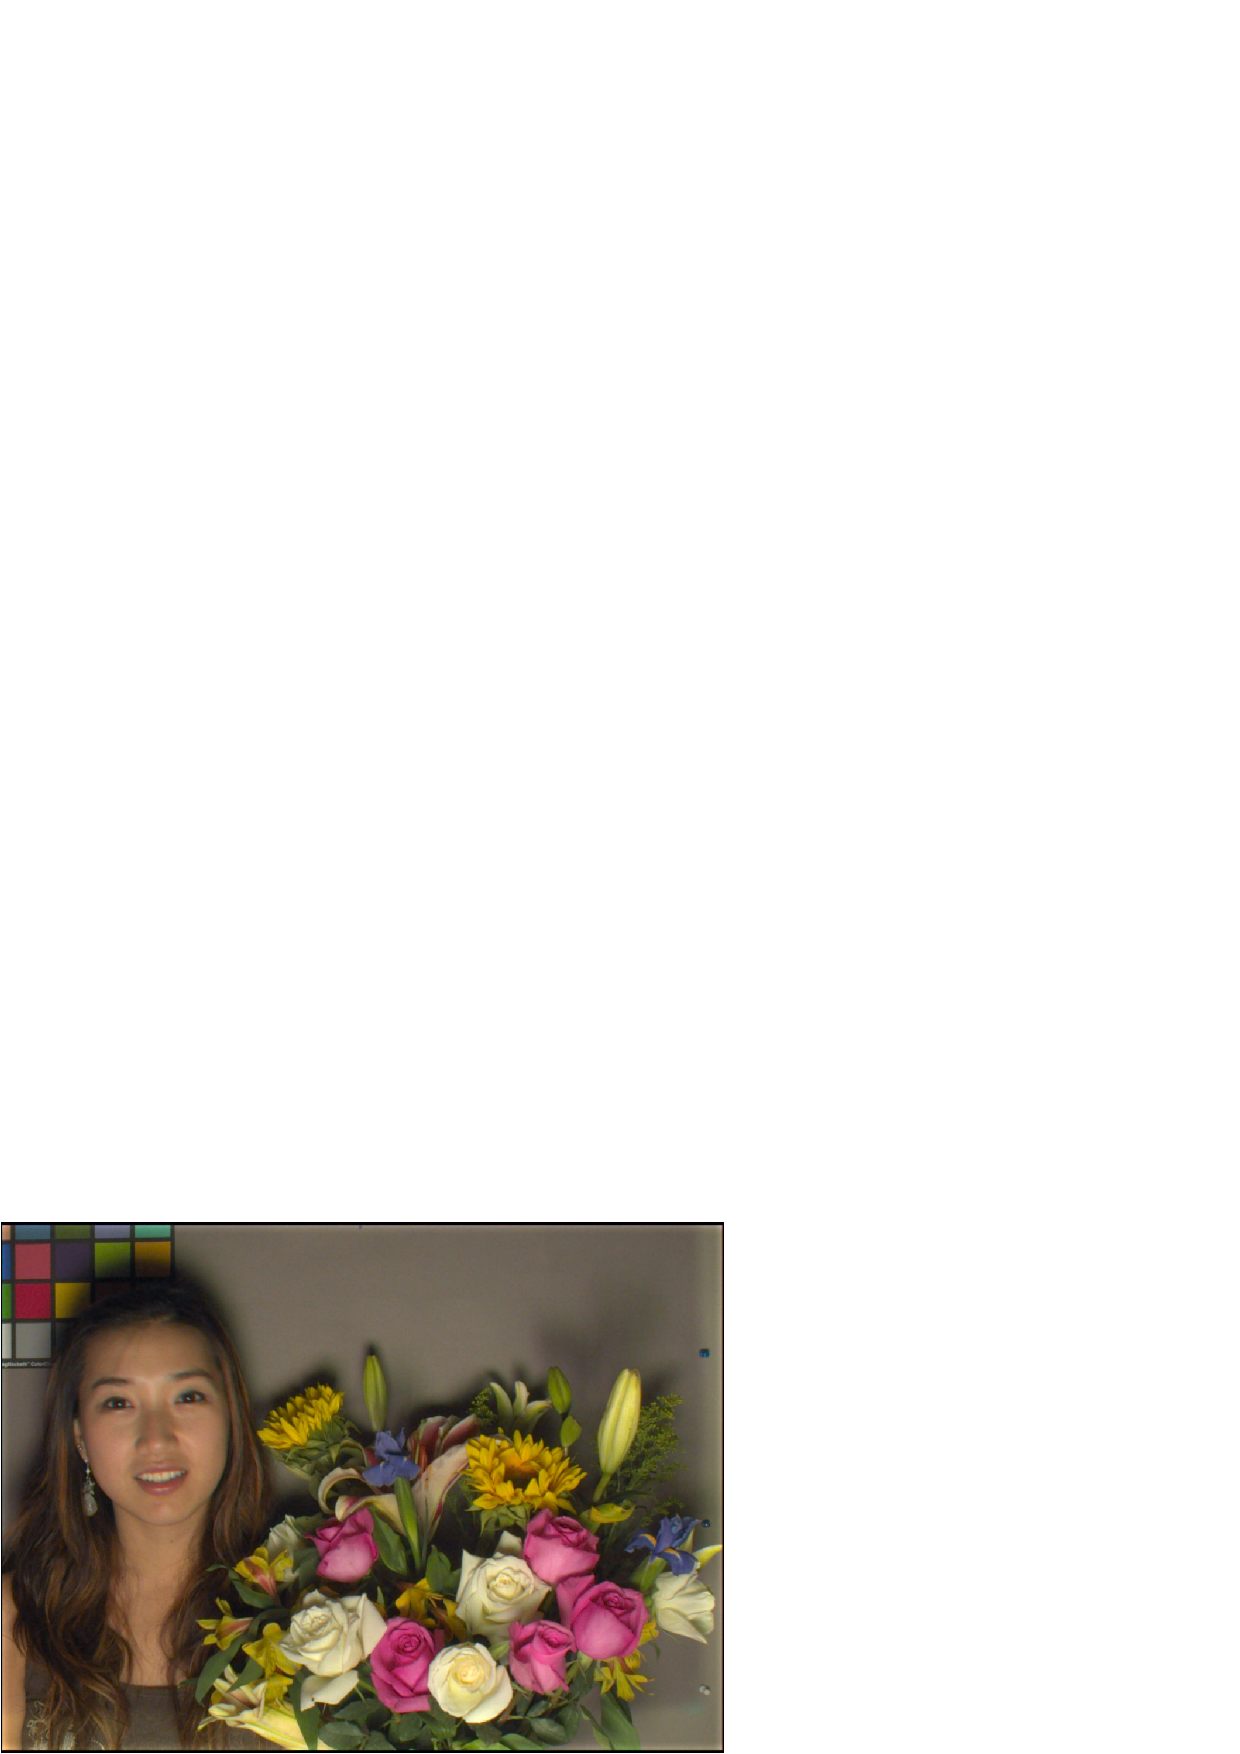
\includegraphics[width=\textwidth]{Fig4/srgbR_AsianFemaleWithFlowers_RGBW1_Fluorescent1_opt3}
 
\includegraphics[width=\textwidth]{Fig4/srgbR_Vegetables_RGBW1_Fluorescent1_opt3}
 \centering\small\text{(d) $\SIDT$}
\end{minipage}
\end{center}
\caption{\textbf{Cross-illuminant and same-illuminant algorithms perform equally well in color rendering for a fluorescent illuminant.} (a) The sensor image under fluorescent, uncorrected. (b) The ideal image under a D65 illumination. (c) A cross-illuminant analysis for the same image but acquired under a fluorescent light. The $\Lcube$ table was built from the fluorescent-acquisition data and XYZ target values for a D65-rendered image. (d) A same-illuminant rendering. In this case the L3 table was built using the same-illuminant D65 table, and the final rendering combined this table with an illuminant correction matrix $\TT$. The cross-illuminant and same-illuminant architectures produce similar images.}
\label{fig:examplesfluorescent}
\end{figure}

We compared the quality of the color rendering using two natural hyperspectral scenes (Figures~\ref{fig:examplestungsten} and \ref{fig:examplesfluorescent}). Each column shows a different representation of the scene. The leftmost columns show the scene as measured under a tungsten illuminant (Figure~\ref{fig:examplestungsten}(a)) and a fluorescent illuminant (Figure \ref{fig:examplesfluorescent}(a)). The scene rendered under a D65 illuminant, calculated from the multispectral data, is shown in panel (b). The original data rendered using $\XI$ table is shown in panel (c), and rendered using the $\SID$ table and linear transformation $\TT$ ($\SIDT$) is shown in (d). The $\XI$ and $\SIDT$ renderings (panels c and d) are good approximations to the calculated D65 rendering (panel b).

\begin {table}[b]
\begin{center}
\begin{tabular}{|l|c|c|}
\hline 
Color reproduction error ($\Delta E$) & Average (Std. dev.) & 90th percentile \\ \hline 
$\XIT$ $\Lcube$ & 2.5 (1.8) & 4.9 \\ 
$\SIT$ $\Lcube$ with linear color transform $\TT$ ($\SITT$) & 2.5 (2.0) & 5.4 \\ 
$\SID$ $\Lcube$ with linear color transform $\TT$ ($\SIDT$) & 4.0 (3.0) & 8.3 \\
$\SIE$ $\Lcube$ with linear color transform $\TT$ ($\SIET$) & 2.9 (2.2) & 6.0 \\\hline 
\end{tabular} 
\end{center}\caption{\textbf{Color reproduction errors ($\Delta E$) for the Natural-100 color chart.} The original images were simulated using a tungsten illuminant. The left column shows the training method used to derive the $\Lcube$ table. The mean reproduction error (middle) and the relatively large reproduction errors (right) are shown. The smallest reproduction error is from the cross-illuminant table. But the errors from several same-illuminant tables followed by a linear transform are only slightly larger.} 
\label{tab:colorErrorTable} 
\end{table}

We quantified the color rendering quality accuracy using the Natural-100 test chart (Table~\ref{tab:colorErrorTable}). The $\XI$ color reproduction errors are very similar to the $\SIGT$ color errors. Hence, the color accuracy of the efficient single-illuminant approach matches the cross-illuminant table for the tungsten illuminant.

Interestingly, we found that the $\SID$ table trained with tungsten illumination can replace the $\SIT$ table with only a small reduction in color reproduction accuracy (1.5$\Delta E$). Using a $\SI$ table derived from training on an ensemble (tungsten and D65) of illuminants reduces the color accuracy by even less (0.4$\Delta E$). As a result, we believe that training a $\SI$ table from data with an ensemble of illuminants may provide the best $\SI$ approach.

\begin{figure}[t]
\begin{center}
\begin{minipage}[b]{0.245\textwidth}
 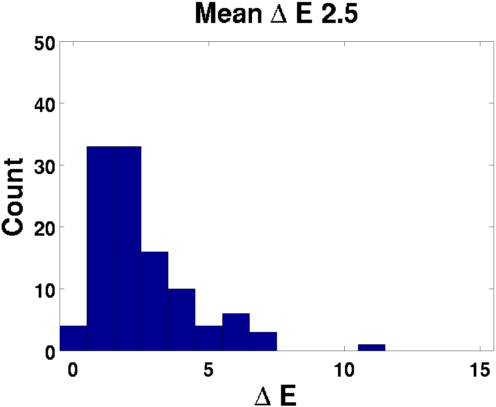
\includegraphics[width=\textwidth,height=\textwidth]{Fig5/Hist15_Tungsten1_RGBW1_2}
 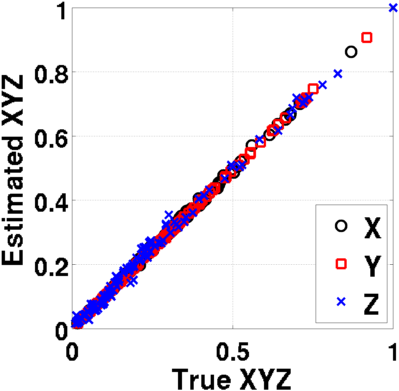
\includegraphics[width=\textwidth]{Fig5/XYZ_Tungsten1_RGBW1_2}
 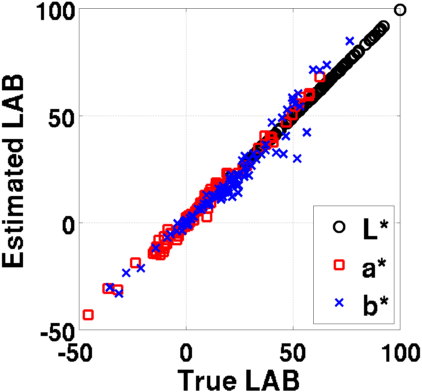
\includegraphics[width=\textwidth]{Fig5/LAB_Tungsten1_RGBW1_2}
 \centering\small\text{(a) $\XIT$}
\end{minipage}
\begin{minipage}[b]{0.245\textwidth}
 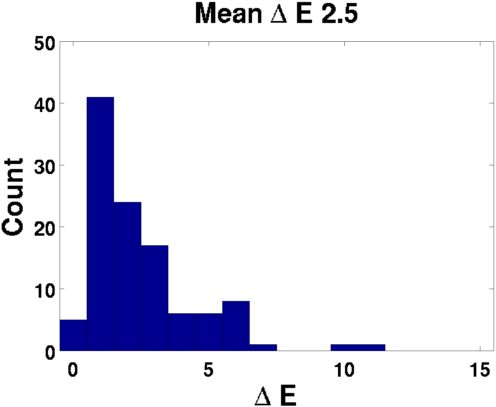
\includegraphics[width=\textwidth,height=\textwidth]{Fig5/Hist15_Tungsten1_RGBW1_6}
 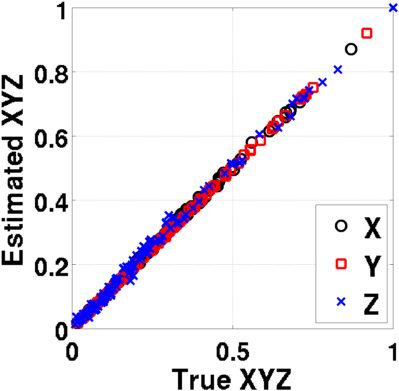
\includegraphics[width=\textwidth]{Fig5/XYZ_Tungsten1_RGBW1_6}
 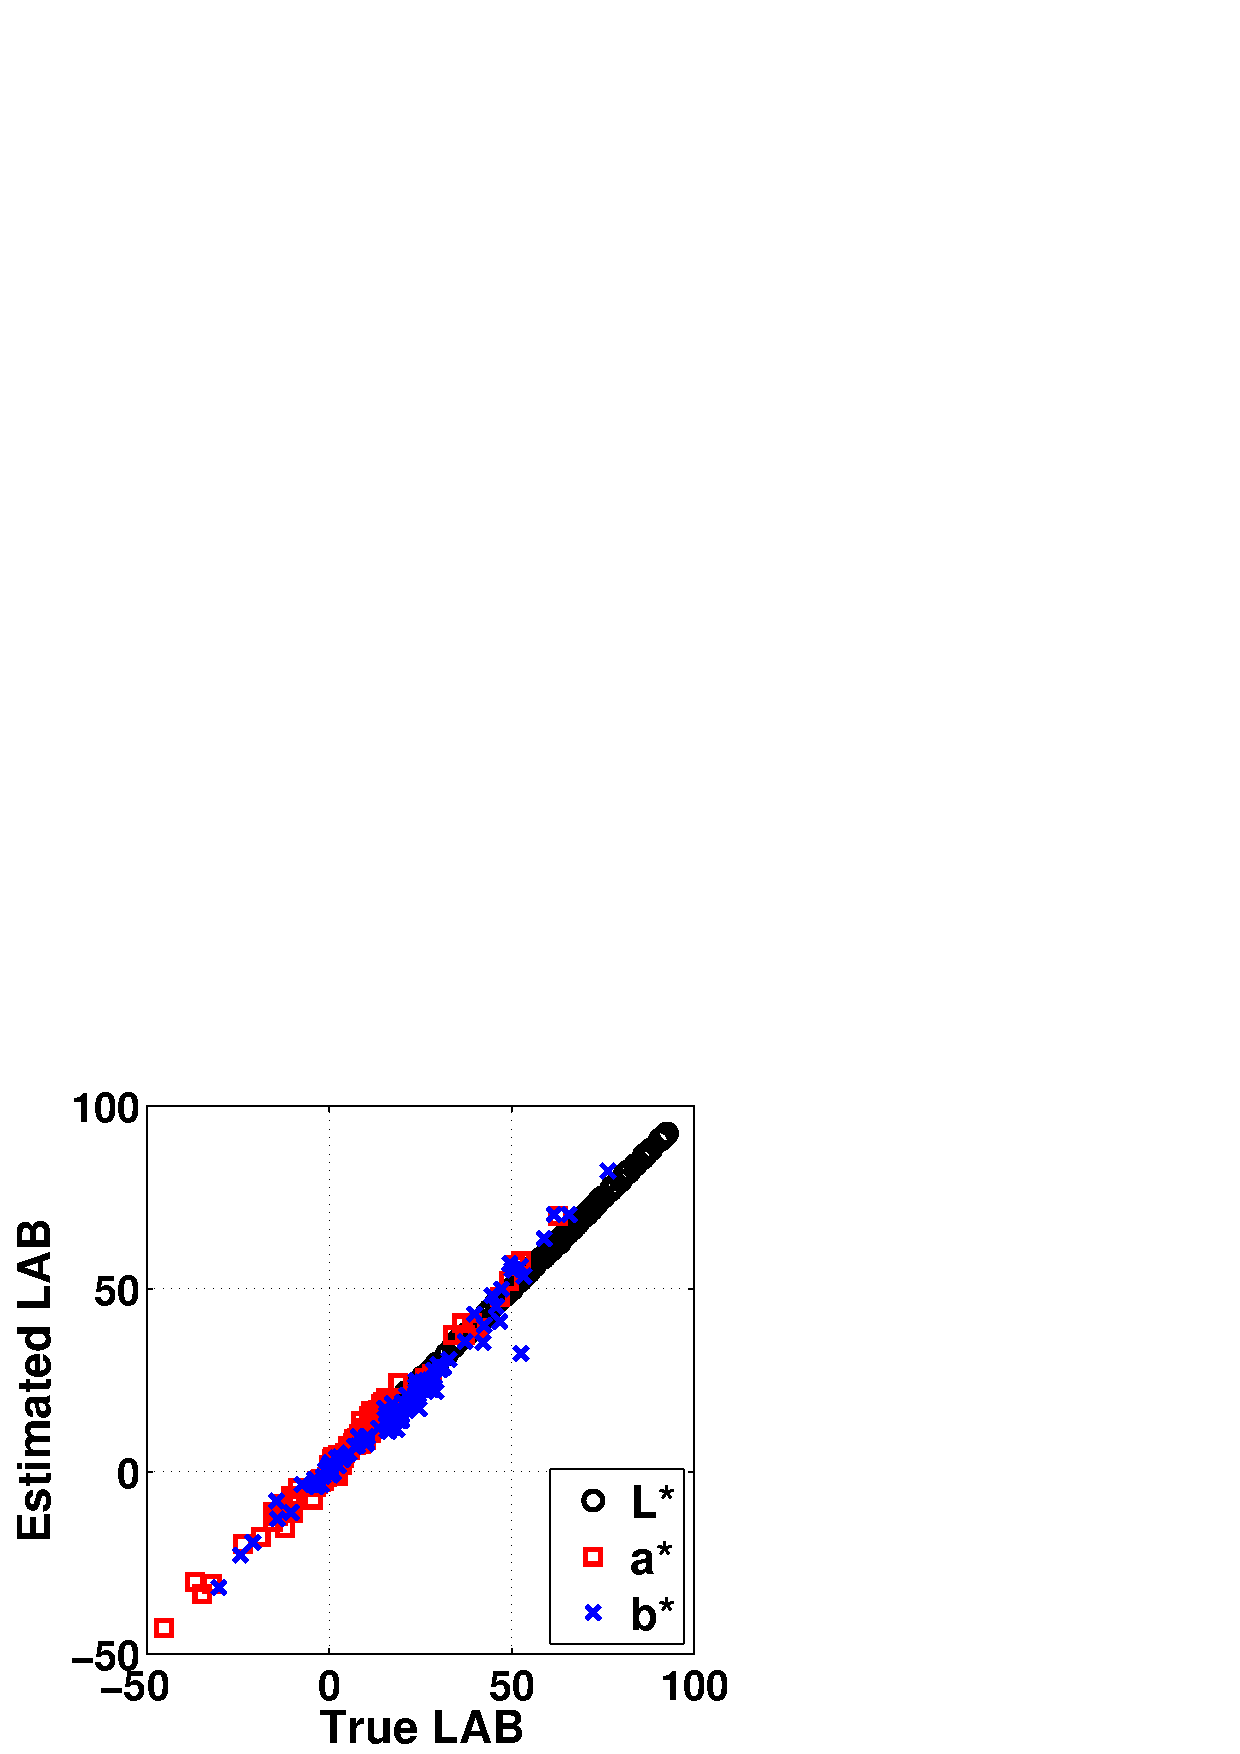
\includegraphics[width=\textwidth]{Fig5/LAB_Tungsten1_RGBW1_6}
 \centering\small\text{(b) $\SITT$}
\end{minipage}
\begin{minipage}[b]{0.245\textwidth}
 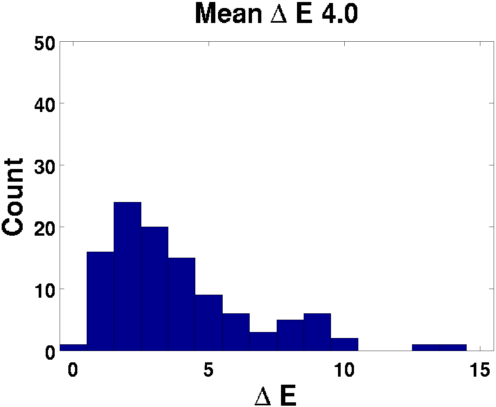
\includegraphics[width=\textwidth,height=\textwidth]{Fig5/Hist15_Tungsten1_RGBW1_3}
 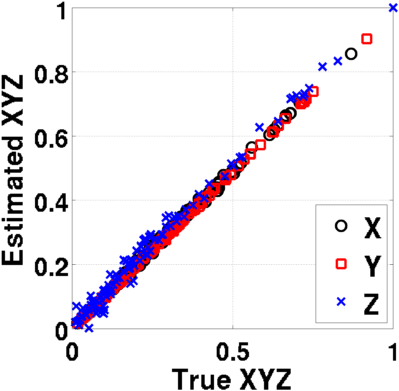
\includegraphics[width=\textwidth]{Fig5/XYZ_Tungsten1_RGBW1_3}
 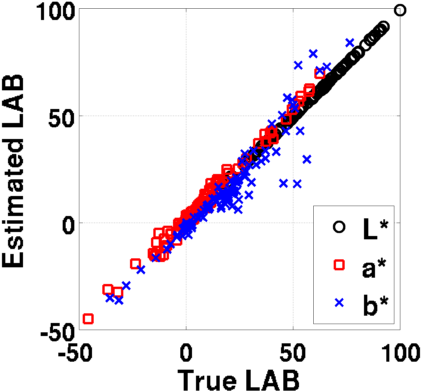
\includegraphics[width=\textwidth]{Fig5/LAB_Tungsten1_RGBW1_3}
 \centering\small\text{(c) $\SIDT$}
\end{minipage}
\begin{minipage}[b]{0.245\textwidth}
 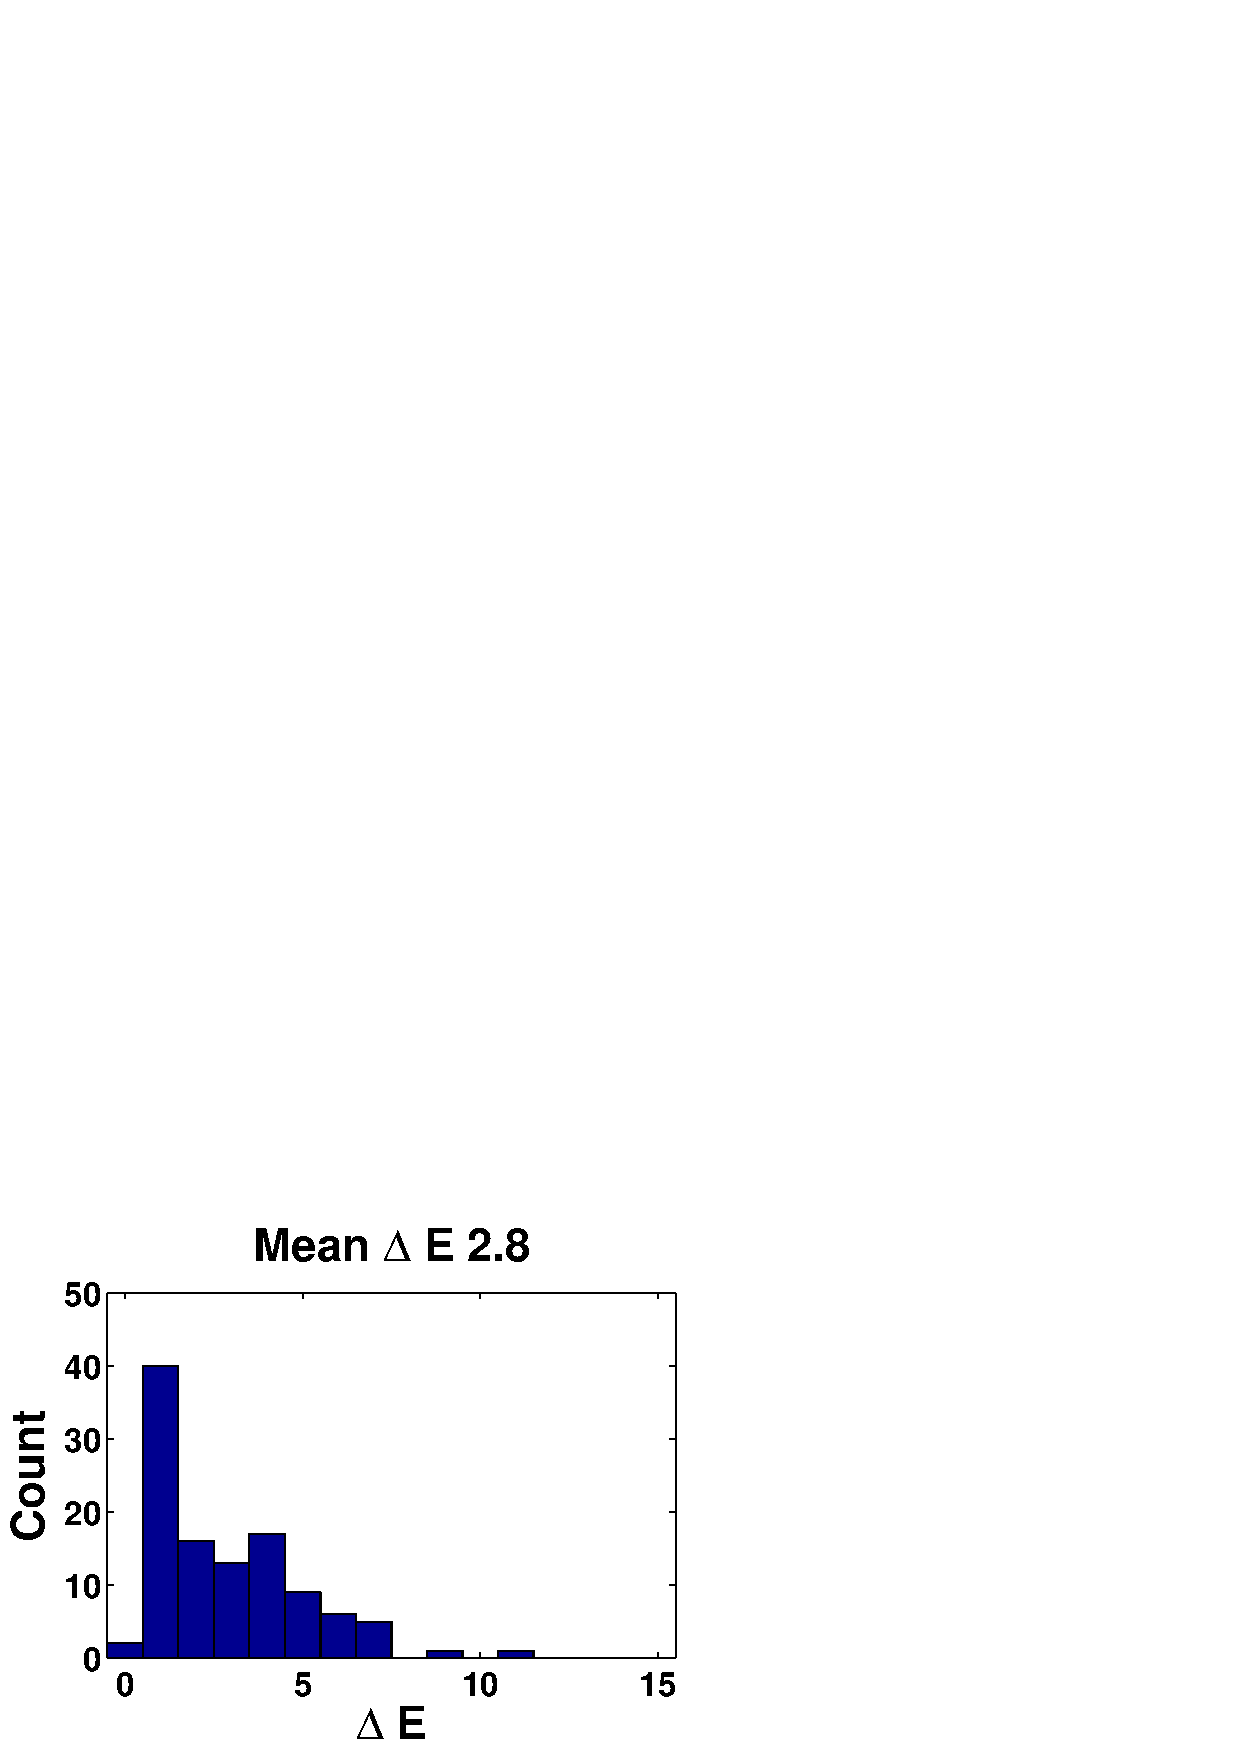
\includegraphics[width=\textwidth,height=\textwidth]{Fig5/Hist15_Tungsten2_RGBW1_6}
 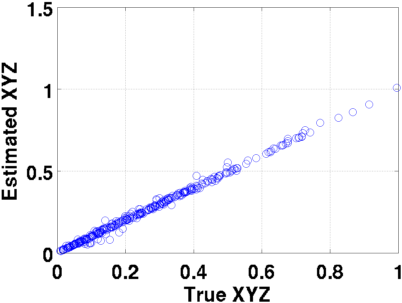
\includegraphics[width=\textwidth]{Fig5/XYZ_Tungsten2_RGBW1_6}
 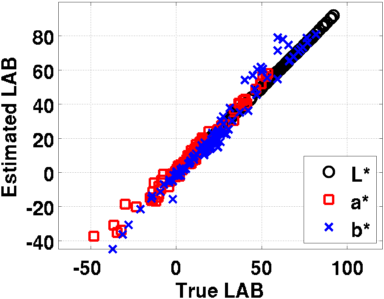
\includegraphics[width=\textwidth]{Fig5/LAB_Tungsten2_RGBW1_6}
 \centering\small\text{(d) $\SIET$}
\end{minipage}
\end{center}
\caption{\textbf{Color error distributions for a Natural-100 chart acquired under a tungsten illuminant and rendered using different $\Lcube$ tables.} We compare the distribution of color reproduction error in $\Delta E$ units (top) and the comparison between true and estimated XYZ (middle) and L*a*b* coordinates (bottom) for the 110 chart reflectances for (a) the cross-illuminant table ($\XIT$), (b) the same-illuminant table trained under tungsten followed by the illuminant transform $\TT$ ($\SITT$), (c) the same-illuminant table trained under D65 followed by the illuminant transform $\TT$ ($\SIDT$) and (d) the same-illuminant table trained under an ensemble of illuminants followed by the illuminant transform $\TT$ ($\SIET$).}
\label{fig:colorStatisticsPlot}
\end{figure}

A more detailed account of the color reproduction error for the cross-illuminant tables ($\XIT$) and two different same-illuminant tables followed by the illuminant transform ($\SITT$ and $\SIDT$) is presented in Figure~\ref{fig:colorStatisticsPlot} with the distribution of the $\Delta E$ values recorded for each reflectance on the Natural-100 chart and the scatter plots comparing the CIE XYZ as well as the L*a*b* color values of the true and reproduced colors.

\section{CONCLUSIONS}

We compared color reproduction accuracy following illuminant correction for two versions of the $\Lcube$ algorithm. In the $\SI$ version we store a single, same-illuminant table and a set of 3 $\times$ 3 illuminant correction transformations. In the $\XI$ version, we store a set of tables, one for each illumination. The $\SI$ method requires far less storage than the $\XI$ method and costs very little in terms of color reproduction accuracy. We present different options regarding the choice of the same-illuminant table. We suggest that the best option for a same-illuminant table might be derived by training the $\Lcube$ algorithm with data simulated using an illuminant ensemble. 

\bibliography{L3}
\bibliographystyle{spiebib}

\end{document}
